\iffalse
\begin{frame}
\frametitle{Isolated Non-word Correction}
\begin{align*}
\textsc{RETRIEVE}:\,& s \in A^n \to \{ w_1, w_2, \ldots, w_m \} \\
\textsc{RANK}:\,& s \in A^n \times \{ w_1, w_2, \ldots, w_m \} \to w_{r_1}, w_{r_2}, \ldots, w_{r_m}
\end{align*}
\end{frame}

\begin{frame}
\frametitle{\textsc{RETRIEVE} Techniques}
\begin{itemize}
\item Near-miss (\texttt{ispell} circa 1970)
\item Phonetic matching 
    \begin{itemize}
    \item SOUNDEX
    \item Metaphone-2
    \item NYSIIS
    \end{itemize}
\item Hybrid  
\end{itemize}
\end{frame}

\begin{frame}
\frametitle{Ranking with String Metrics} 
\begin{itemize}
\item Levenshtein distance
\item Damerau-Levenshtein distance
\item Jaro-Winkler distance
\end{itemize}
\end{frame}

\begin{frame}
\frametitle{Random Forest \textsc{RANK}}
\footnotesize
\input figures/chapter04/random-forest-features.tex
\end{frame}
\fi

\begin{frame}
\frametitle{Isolated Non-word Error Correction Data}
\centering
\begin{tabular}{cccc}
\textsc{Non-word} & \textsc{Candidate} & \textsc{Target} & \textsc{Jaro-Winkler} \\
\hline
{\string^}hifin\$ & {\string^}haven\$    & 0 & .60 \\
{\string^}hifin\$ & {\string^}hyphen\$   & 1 & .58 \\
{\string^}hifin\$ & {\string^}heaven\$  & 0 & .58 \\
{\string^}hifin\$ & {\string^}Havana\$   & 0 & .46 \\
\end{tabular}
\end{frame}

\begin{frame}
\begin{figure}
\input figures/chapter04/isolated-nonword-binary-cosine.tex
\end{figure}
\end{frame}

\begin{frame}
\begin{figure}
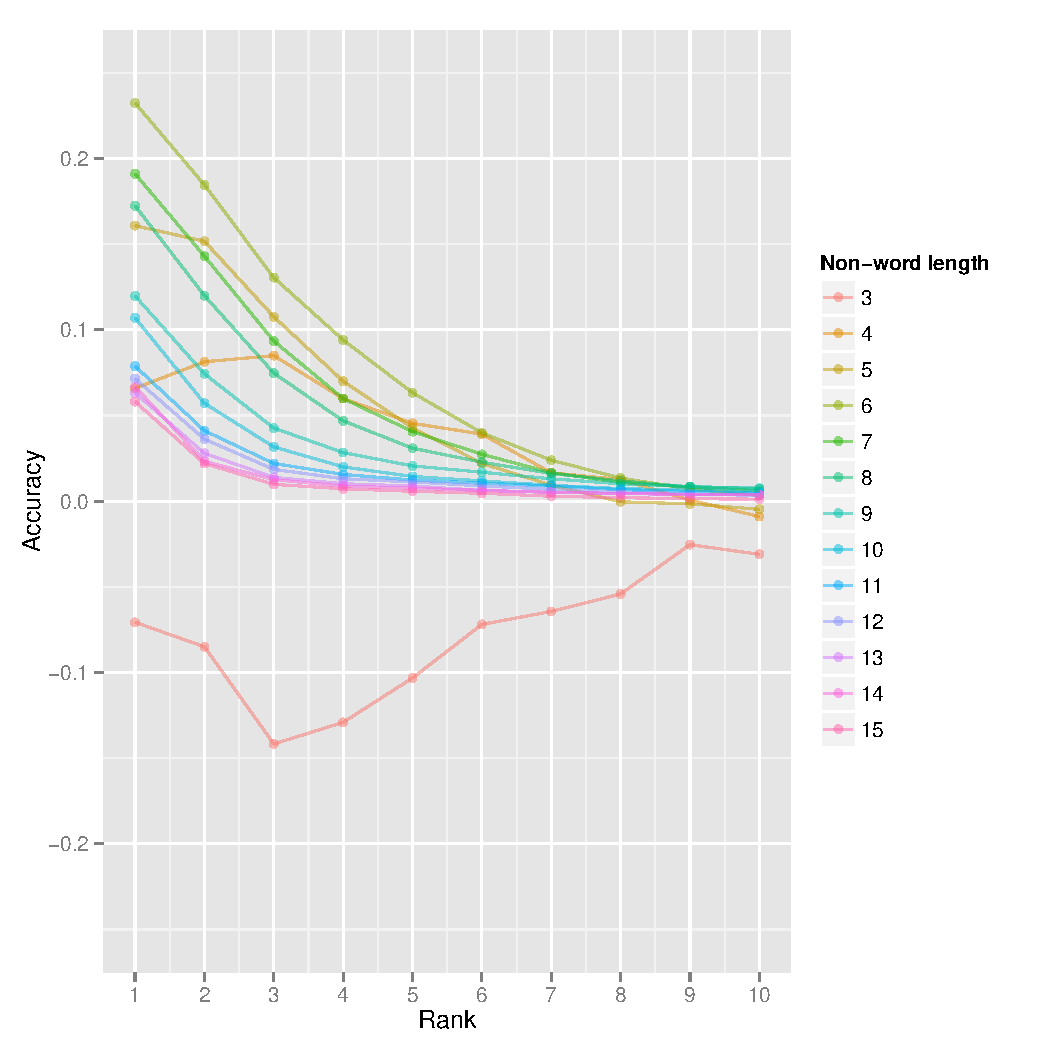
\includegraphics[height=\textheight]{figures/chapter04/ranks-by-length-difference}
\end{figure}
\end{frame}

\begin{frame}
\begin{figure}
\small
\input figures/chapter04/accuracy-at-k-mitton-binary.tex
\end{figure}
\end{frame}

%\begin{frame}
%\begin{figure}
%\small
%\input figures/chapter04/accuracy-at-k-mitton-multiclass.tex
%\end{figure}
%\end{frame}